\documentclass[12pt]{article}
\everymath{\displaystyle}
\usepackage{unicode-math}
\usepackage{pgfplots}
\pgfplotsset{compat=1.18}
\usepackage{amsmath}



\usepackage[margin=1in]{geometry}
\usepackage{tcolorbox}
\usepackage{graphicx}
\usepackage{tikz}
\usepackage{amssymb}
\usepackage{enumitem}
\usepackage{titlesec}
\usepackage{fancyhdr}
\usepackage{pifont}
\usepackage{xcolor}
\newcounter{questionnum}
\setcounter{questionnum}{0}
\usepackage{eso-pic} % for page background

% --------- 主题颜色设置 ---------
\definecolor{novelblue}{RGB}{70,60,150}
\definecolor{headerbg}{RGB}{240,240,255}

\pagestyle{fancy}
\fancyhf{}
\renewcommand{\headrulewidth}{0.4pt}
\renewcommand{\headrule}{\hbox to\headwidth{\color{novelblue}\leaders\hrule height 0.4pt\hfill}}

% --------- 页眉背景色条 ---------
\newcommand{\headbackground}{
  \AddToShipoutPictureBG*{
    \begin{tikzpicture}[remember picture, overlay]
      \fill[blue!5!purple!10] (current page.north west) rectangle ([yshift=-60pt]current page.north east);
    \end{tikzpicture}
  }
}

% --------- 页眉设置 ---------
\pagestyle{fancy}
\fancyhf{}
\renewcommand{\headrulewidth}{0pt}
\fancyhead[L]{\color{novelblue}\textbf{\textbf{Novel Prep} }}
\fancyhead[C]{\color{novelblue}\textbf {SAT Preparation}}
\fancyhead[R]{\color{novelblue}\textbf{Jack Zeng}}


\newtcolorbox{SATCard}[1][]{%
  enhanced,
  colback=white,
  colframe=novelblue,
  coltitle=white,
  boxrule=0.6pt,
  arc=4pt,
  boxsep=5pt,
  left=8pt, right=8pt, top=10pt, bottom=10pt,
  sharp corners=south,
  drop shadow south east,
  #1
}

% --------- 顶部 Mark for Review 栏 ---------
\newcommand{\markforreview}{
  \stepcounter{questionnum} % 自动递增题号
  \begin{tikzpicture}[scale=1.1]
    % 黑色题号
    \fill[black] (0,0) rectangle (0.8,0.6);
    \node[white, font=\bfseries\large] at (0.4,0.3) {\thequestionnum};

    % 灰底主栏
    \fill[gray!10] (0.8,0) rectangle (14.5,0.6);

    % Mark for Review
    \node[anchor=west, font=\small] at (1.2,0.3) {\ding{72} \hspace{2pt}Mark for Review};

    % ABC 按钮区域
    \draw[thick, rounded corners=3pt] (13.5,0.12) rectangle (14.5,0.48);
    \node[font=\bfseries\normalsize] at (14.0,0.3) {ABC};
  \end{tikzpicture}


  \newcommand{\choiceboxcircled}[2]{%
  \begin{tcolorbox}[
    colback=white,
    colframe=black,
    boxrule=0.5pt,
    rounded corners=6pt,
    left=6pt, right=6pt, top=6pt, bottom=6pt,
    width=\linewidth
  ]
    \textbf{\large\textcircled{\textbf{#1}}} \ #2
  \end{tcolorbox}
}
}

% --------- 选项框样式 ---------
\newcommand{\choicebox}[2]{%
  \begin{tcolorbox}[
    colback=white, 
    colframe=novelblue,
    boxrule=0.5pt, 
    rounded corners=4pt, 
    left=6pt, right=6pt, top=6pt, bottom=6pt,
    width=\linewidth
  ]
  \textbf{#1.} \ #2
  \end{tcolorbox}
}


\begin{document}
\section*{SAT Hard Question 14}
\noindent\markforreview
\vspace{1em}

For two acute angles, \(\angle Q\) and \(\angle R\), \(\cos(Q) = \sin(R)\).  
The measures, in degrees, of \(\angle Q\) and \(\angle R\) are \(x + 61\) and \(4x + 4\) respectively.  
What is the value of \(x\)?

\vspace{2em}
\noindent\markforreview
\vspace{1em}

If \(a\) and \(b\) are numbers greater than 1 and \(\sqrt[7]{a^6}\) is equivalent to \(\sqrt{b^3}\),  
for what value of \(n\) is \(a^{2n+1} = b\)?

\vspace{2em}
\noindent\markforreview
\vspace{1em}

The function \(c\) gives the partial length, in centimeters (cm), of the circumference of a circle with radius \(r\) cm:  
\[
c(r) = \frac{2}{5}(2\pi r)
\]  
For each increase of 18 cm in \(r\), this partial length increases by \(k\pi\) cm.  
What is the value of \(k\)?

\vspace{2em}

\noindent\markforreview
\vspace{1em}

For each real number \(r\), which of the following points lies on the graph of both equations in the \(xy\)-plane for the given system?

\[
\begin{aligned}
15x + 45y &= 33 \\
5x + 15y &= 11
\end{aligned}
\]

\choicebox{A}{\(\left( \frac{11r}{5} - 3, r \right)\)}  
\choicebox{B}{\(\left( -3r + \frac{11}{5}, r \right)\)}  
\choicebox{C}{\(\left( r, -\frac{r}{3} - \frac{11}{15} \right)\)}  
\choicebox{D}{\(\left( r, \frac{r}{3} + \frac{11}{15} \right)\)}

\vspace{2em}

\newpage

\noindent\markforreview
\vspace{1em}

If \(\frac{a}{b} = \frac{4}{5}\) and \(\frac{5b}{ta} = 35\), what is the value of \(t\)?

\vspace{2em}

\noindent\markforreview
\vspace{1em}

In the given equation, \( c \) is a constant.  
If the equation has exactly one solution, what is the value of \( c \)?  
\[
\frac{1}{2cx} = \frac{x}{16} + \frac{1}{c}
\]


\noindent\markforreview
\vspace{1em}

The given equation is one equation in a system of two linear equations.  
If the system has at least one solution, which of the following equations could be the other equation in the system?  
\[
7x + 5y = 2
\]

\noindent I. \(10.5x + 7.5y = 3\)  

\noindent II. \(10.5x - 7.5y = 3\)

\choicebox{A}{I only}  
\choicebox{B}{II only}  
\choicebox{C}{I and II}  
\choicebox{D}{Neither I nor II}

\vspace{2em}
\noindent\markforreview
\vspace{1em}

The function \( f \) is defined by \( f(x) = a^x - b \), where \( a \) and \( b \) are constants.  
In the \(xy\)-plane, the graph of \( y = f(x) \) passes through the points \( (c, 7) \) and \( (2c, 117) \), where \( c \) is a constant.  
Which of the following could be the value of \( b \)?
\newpage

\noindent\markforreview
\vspace{1em}

A right rectangular prism has a base area of \(16t\) square centimeters (\(\text{cm}^2\)).  
The length of the base of the rectangular prism is \( \frac{8}{3} \) cm, and the height of the prism is 9 cm.  
Which expression represents the surface area, in \(\text{cm}^2\), of the right rectangular prism?

\vspace{2em}
\noindent\markforreview
\vspace{1em}

The mass of object \( A \) is 498\% of the mass of object \( B \),  
and the mass of object \( A \) is 0.830\% of the mass of object \( C \).  
If the mass of object \( C \) is \( p\% \) of the mass of object \( B \), what is the value of \( p \)?
\vspace{2em}

\noindent\markforreview
\vspace{1em}

Which of the following expressions has a factor of \( x + 2b \),  
where \( b \) is a positive integer constant?

\choicebox{A}{\(3x^2 + 7x + 14b\)}  
\choicebox{B}{\(3x^2 + 16x + 14b\)}  
\choicebox{C}{\(3x^2 + 18x + 14b\)}  
\choicebox{D}{\(3x^2 + 25x + 14b\)}

\newpage


\noindent\markforreview


\begin{center}
    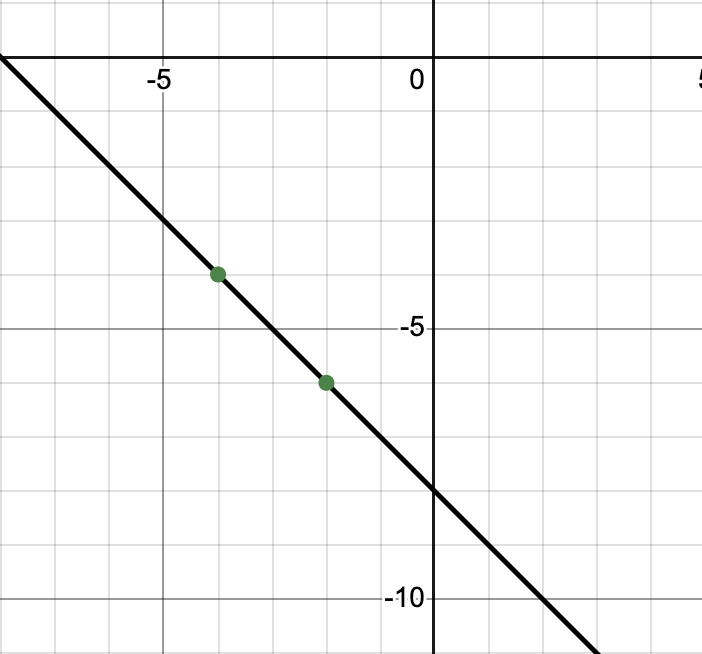
\includegraphics[width=0.4\linewidth]{f10.png}
\end{center}

The graph of the linear function \( y = f(x) - 19 \) is shown.  
If \(c\) and \(d\) are positive constants, which equation could define \(f\)?

\choicebox{A}{\(f(x) = d - cx\)}  
\choicebox{B}{\(f(x) = -d + cx\)}  
\choicebox{C}{\(f(x) = d + cx\)}  
\choicebox{D}{\(f(x) = -d - cx\)}

\vspace{2em}
\noindent\markforreview
\vspace{1em}

The expression \(kx\) represents the result of decreasing a positive force, \(x\), acting on  
an object by \(0.34\%\).  
What is the value of \(k\)?

\choicebox{A}{\(0.34\%\)}  
\choicebox{B}{\(1.34\%\)}  
\choicebox{C}{\(99.66\%\)}  
\choicebox{D}{\(100.34\%\)}

\vspace{2em}
\newpage
\noindent\markforreview
\vspace{1em}

A regular polygon has exactly 87 sides. If the measure of each of the 87 interior angles of  
this polygon is \((180p)^\circ\), what is the value of \(p\)?

\choicebox{A}{\(\frac{85}{87}\)}  
\choicebox{B}{\(\frac{37}{87}\)}  
\choicebox{C}{\(\frac{87}{90}\)}  
\choicebox{D}{\(\frac{87}{180}\)}

\vspace{2em}

\noindent\markforreview
\vspace{1em}

The function \( f(n) = 7(20.44)^{\frac{n}{4}} \) gives each term of a sequence as a function of the term’s position \( n \) in the sequence, where \( n \) is a whole number.  
The value of the term in position 14 is \( p\% \) more than the value of the term in position 10.  
What is the value of \( p \)?

\vspace{2em}

\noindent\markforreview
\vspace{1em}

A right square pyramid has a total surface area of 28,160 square inches, and the combined surface area of the four lateral faces of this pyramid is 16,060 square inches.  
What is the height, in inches, of this pyramid?

\choicebox{A}{\(48\)}  
\choicebox{B}{\(55\)}  
\choicebox{C}{\(73\)}  
\choicebox{D}{\(110\)}

\vspace{2em}
\newpage
\noindent\markforreview
\vspace{1em}

In the given equation, \(k\) is a constant. The equation has exactly one real solution.  
What is the minimum possible value of \(4k\)?

\[
\sqrt{k - x} = 32 - x
\]

\vspace{2em}












\end{document}